\documentclass[palace_of_the_silver_princess]{subfiles}

\begin{document}
\fontfamily{ppl}\selectfont
\clearpage

\twocolumn[{\section{Part 2: Dungeon Master's Information}}]
\markright{Part 2: Dungeon Master's Information}

The information given below should be read carefully. Part of it can be
given to players. It will be up to the DM to decide exactly what the
players should know about the palace. This information can be altered if
desired. The DM is encouraged to add whatever he or she wants to this
information to give more color to the palace.

The dead soldiers found on the entrance level are from an unnamed army.
It will be up to the DM to decide where they came from, why they are in
the palace and any other information concerning the dead soldiers. They
could be from a lost city; from a hidden fortress of highly skilled
thieves and fighters; or from a forgotten race or tribe of people. The
DM could even have these soldiers be a scouting party for a larger
brigade who plan on taking the ruined palace and making it a fort or
base station from which to work. The possibilities are as endless as the
imagination of the DM.

The dungeon is constructed of marble. The doors are of iron-reinforced
oak. The passageways are fairly clean due to the gelatinous cube that
roams the hallways. All passageways are 10’x10’.  Torch sconces are
mounted every ten feet along all the passageways on alternating sides.
None have torches. Arrases will frequently be seen throughout the palace
as well as pots of dead plant life.

\subsection{Legend}

Ancient legends of the land speak of a beautiful young princess called
Argenta who lived in a wonderful enchanted palace made of every type of
marble known. Her palace was in the heart of a rich, fertile valley
filled with gentle creatures that could do no harm.  Exotic flowers and
plant life grew everywhere, water ran sweet and clear and the skies were
always clear and warm.

Mica flickered in all the rocks and was often found in the streams
making them glisten like diamonds in the bright sunlight. Early morning
dew drops clung gently to leaves of small trees and grass, appearing
like fairy jewels scattered from wild dance the night before. Wild birds
with long, colorful tails and bright faces filled the air with the sweet
sounds of their love songs. Tiny animals freely darted in and out of the
underbrush, fearing nothing, as there were no enemies anywhere to be
found. The dwarves that lived in the valley loved Princess Argenta very
much. They worked her silver and ruby mines so that the elves who shared
the valley with them could make beautiful jewelry and weapons.
Everything in the valley was peaceful.

One day, according to legend, a ruby the size of an apple was found.  A
perfect ruby. The dwarves cut the ruby carefully so that its size would
not be diminished. The elves polished the ruby until it shone so that it
was almost impossible to gaze upon. They presented it to the princess
and told her that it was as lovely as she, and they called it "My Lady’s
Heart". So pleased was the princess that she decided to honor her
friends, the elves and dwarves, with a grand party; a masquerade ball.
Everyone was invited to come.

One the eve of the grand ball, people poured into the valley from
everywhere. How so many people had heard about the party no one knew,
but the princess did not mind. She was proud of the ruby and wanted
everyone to see “My Lady’s Heart”. She should not have been so eager to
show the ruby, as one guest was interested in more than its beauty
alone. He had come to steal it. His eyes also roamed freely to the
princess, and he gazed upon her as much as he gazed upon the brilliant
gem. Princess Argenta saw this, and in her innocence smiled backed at
him. Two dwarves and an elf saw this, and when they challenged him after
the party, they were never seen or heard from again.

Many weeks after the party a red dragon was seen in the skies of the
valley. The dragon burned the rich land with its breath and terrorized
the gentle people of the valley. The land was left scorched and barren.
Those valley people unfortunate to get close enough to the dragon (but
fortunate enough to live) swore that they saw a man in silver and blue
armor riding on its back.  Some folks still say that they see a red
dragon in the skies over the valley. Many say that they see a saddle on
the dragon’s back and loose reins near its head.

The valley is now dead, the palace is in ruins. No one knows exactly
what happened to the princess. Some believe that the man on the dragon
carried her away. Others think that he killed her and stole what
treasure he could find. But all stories say that the ruby, “My Lady’s
Heart,” is still hidden in the palace.

\subsection{Lands, Cities, and Villages}

The information given below describes the surrounding lands near the
Palace of the Silver Princess in the land of the Princes of Glantri. A
brief outline of each village is given, including its size and what the
life is like there. There is one Barony, and this seat of rulership
controls most of the area. Further information about the surrounding
land may be added by the DM where and when desired.

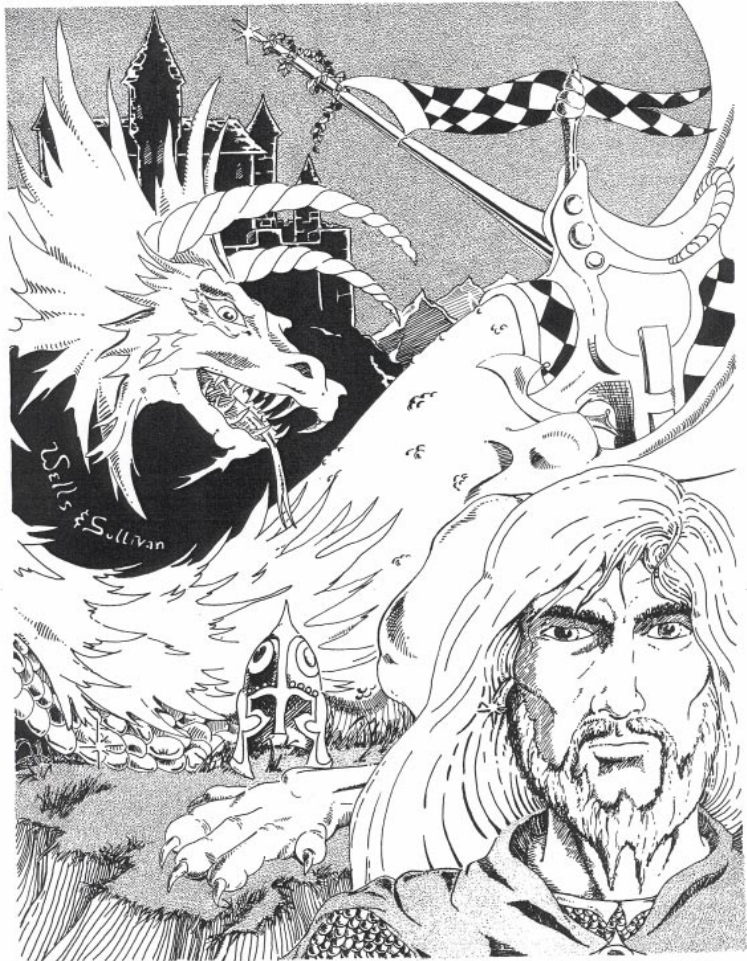
\includegraphics[width=\columnwidth]{img/pic1.png}

As play continues and the characters advance beyond 3rd level, the DM
may plan adventures into the neighboring wilderness, as a break from
dungeon adventures or as part of a dungeon adventure.  Remember,
characters must travel through the mountains and wilderness before
actually reaching the palace ruins. However, DMs are urged not to
attempt wilderness adventures until players have reached expert level
and are now using the D\&D® Expert game rules.

\subsubsection{Gulluvia}

This is a ruthless place filled with terror. The ruler of this chaotic
nightmare is Lady D’hmis. She rules this barony with a firm and
unforgiving hand. To gain supreme rulership of the tiny barony, she
killed her husband. A prime example of the type of laws her ladyship
favors is one forbidding males, except those in her service, from being
on the streets after the sunset unless accompanied by a female who is
age 15 or older. This law meets little resistance as everyone fears her
baronial guards. Though D’hmis’ warriors are primarily male, her
commanders are all females; tough, chaotic women who instill fear by a
mere gaze and who fear little save D’hmis and the elite male fighters
who serve as her personal bodyguards and paramours.

\subsubsection{Dead Mule}

This little shire was once a peaceful place, named by the group of
miners who settled here after their pack mule died.  The shire is now
occupied by Gulluvian soldiers, and no one in the shire seems to know
why. All they know is that soldiers camp outside the shire, and
occasionally terrorize the surrounding countryside. If the mayor knows
why the soldiers are here, he isn’t saying.

\subsubsection{N'Sau}

This small farming village is still untouched by the cruel hand of
D’hmis. The village is so small that there is no tavern or inn here. A
small general store doubles as a tavern or meeting hall when needed. The
main crop grown here is wheat.

\subsubsection{Thorold}

This lovely little village prides itself on the fact that it raises the
best thoroughbred horses in all of Glantri for the Barony of Gulluvia.
Thorold, though it appears peaceful and perhaps even lawful, is just as
chaotic as Gulluvia. The mayor of Thorold is a distant cousin of D’hmis,
and follows her laws and orders to the letter. The village is rather
large and has three taverns, a general store, and two smithies.

\subsubsection{Mere}

This tiny village is primarily inhabited by halflings, though human
folk, elves and dwarves live here too. This village is also under the
protection of Gulluvia, but because it is located so near the Misty
Swamp, D’hmis has little to do with it except at tax time, which is
every three months. Escaped slaves and prisoners come here to equip
themselves before journeying north through the swamp. Mereians say
nothing about the slaves or prisoners, fearing that D’hmis would send
guards to their village to catch them (and they want as little to do
with Gulluvia as possible). This village has two taverns, one general
store, and an inn.

\subsubsection{Velders}

This canton is under the protection of Gulluvia, though this does
Velders little good. The Gulluvian guards fear the Abaddon Woods and do
not like to travel through it to reach Velders except in large groups.
Orcs, kobolds and other vile creatures make periodic raids on the small
farms on the outskirts of the canton.  There is only a trading post in
the center of town.

\subsubsection{Misty Swamp}

No one knows exactly what lies behind the veil of
ever present mist that hovers over the swamp. Some old timers say
that the dwarves who make Anterian Brandy live in the swamp near
their secret ingredient, the swamp water. This is speculation, as no
one really knows what the secret ingredient of Anterian Brandy is.
Others whisper tales of an evil wizard living there in a massive
tower of shiny black stone. Sometimes, in the dead of winter, fierce
thunderstorms can be heard near the swamp, but no one ever sees
any lightning. The only thing people who live near the swamp will
agree on is that most magic users and elves had best stay clear of it
or they will find that their spells will not function properly. One
young magic user tried to catch a rabbit with a web spell near the
swamp one day and ended up with dozens of rabbits, all neatly
webbed, scattered about her feet. She didn’t really mind having the
extra rabbits, but the fact that she couldn’t control her magic
scared her (as it does many other spell casters). She was one of the
fortunate ones; others have not been so lucky.

Once a band of daring adventurers ignored warnings not to venture into
the swamp. Months later only the cleric returned. He told tales of their
battle against creatures made of colored mist, and others that had no
visible form at all. He said they constantly fought strange looking
creatures with three heads, three arms, and three legs. He told of how
their brave elf attempted to cast a {\textbf magic missile} at a beast
who was attacking one of the fighters. Suddenly, however, the elf
changed into a rhinoceros and wandered away into the swamp. Before any
more information could be obtained from the cleric he died. No wounds
could be found, and the folks who found him swear he must have been
scared to death.

The DM can choose how any given spell cast in the swamp will be changed.
The effects should be unexpected by the players, but instant-death
results should {textbf not} be used. Suggested effects are:

\begin{enumerate}
	\item Spell backfires on the caster of the party
	\item Spel fails: nothing happens
	\item Caster throws a different spell of the same level
	\item Spell effect is tripled
	\item Caster or a member of the party glows for 24 hours
	\item Caster or a party member changed into a creature with hit dice
		equal to the character’s level: lasts 24 hours
\end{enumerate}

If the D\&D® Expert rules are also being used, effects like 5 and 6 can
be removed (once the party has left the swamp) by using a dispel magic
spell.

\subsubsection{Abaddon Woods}

This is a desolate place inhibited by evil beings, but was once believed
to be filled with unicorns, elves, faeries and other fair creatures.
Many expeditions attempting to destroy the evil lurking here have
ventured into the woods, but have never returned.

\subsubsection{Moorfowl Mountains}

This ugly, dead, tall range forms a protective shield that keeps the
mist from Misty Swamp from spreading into the neighboring farmlands.
Most folks don’t venture into the mountains much any more except to hunt
for certain types of moss used by local healers. Evil creatures now roam
the mountains freely and inhabit the mines once worked by the dwarves
who served the Silver Princess. These mines now are barren and not worth
working.

\subsubsection{Thunder Mountains}

These low pine-covered mountains see the sunlight infrequently. Most of
the time thick storm clouds linger on the mountain tops — clouds that
often erupt into violent thunder storms. An evil wizardess is rumored to
live in the mountains in a giant hollow oak she uses as a lab. It is
believed that it is she who keeps the thunder storms alive, partly
because she fears the light and partly because it keeps away the
curious. Local people don’t recall anyone ever going into the mountains,
and if anyone ever did, they never returned to tell about it.

\clearpage
\begin{center}
	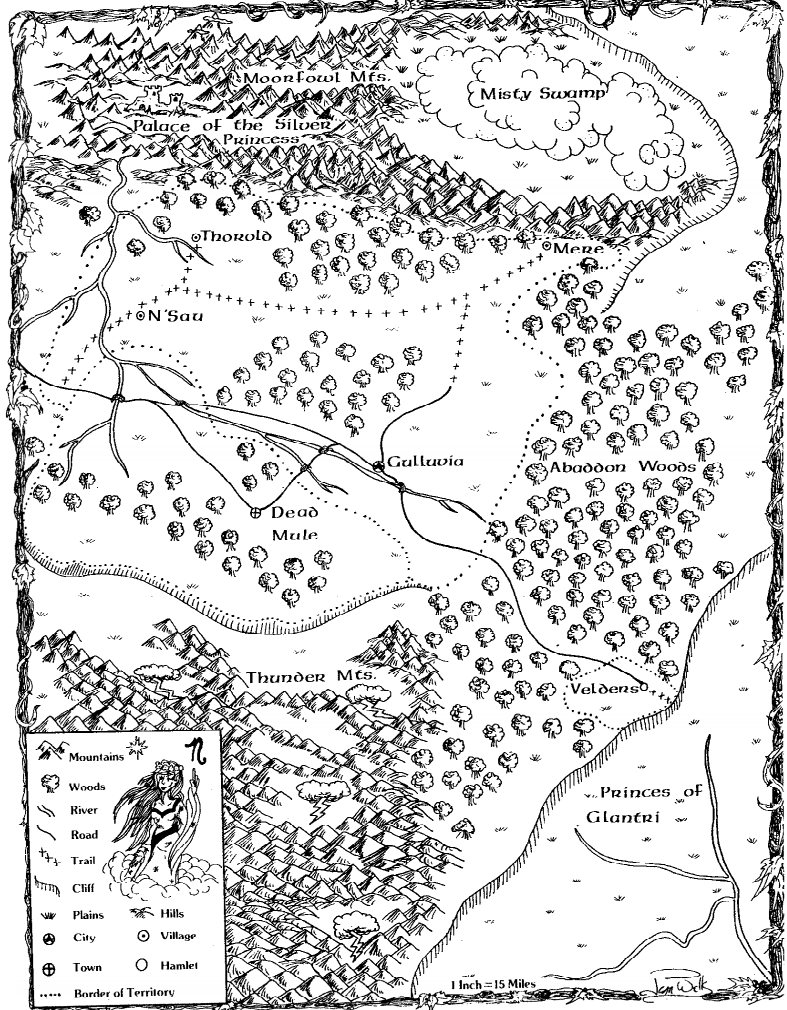
\includegraphics[width=0.9\textwidth]{img/overland_map.png}
\end{center}
\clearpage

\newpage
\begin{figure*}[!ht]
	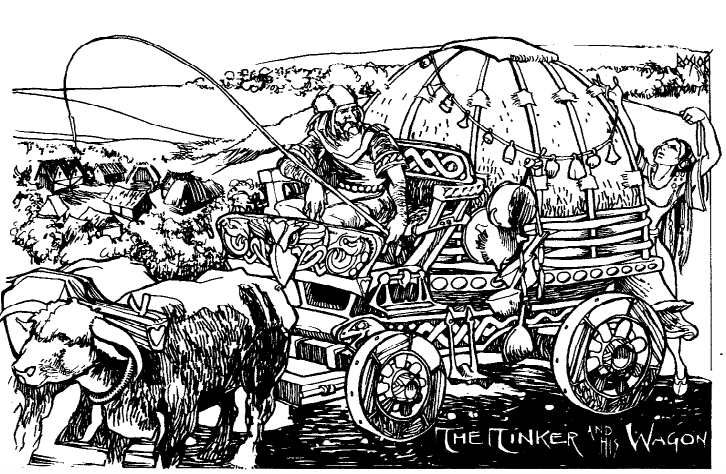
\includegraphics[width=\textwidth]{img/wagon.png}
\end{figure*}

\subsection{The Tinker and His Daughter}

A small tinker’s shop located in Gulluvia is run by an old man and his
daughter. The tinker is a jovial fellow called Lamdomon, who, though
aged, still retains his youthful thick white hair and clear steel blue
eyes. His daughter, a shy girl, rather plain, but not unattractive,
keeps house and runs most of his errands. She is called Zappora. Her
fiery red hair falls just to her waist and her green eyes, says
Lamdomon, shame even the brightest forest. Zappora is very superstitious
and will never do anything that might bring bad luck or invite evil
spirits. She always carries a pair of dice, a package of salt, a bud of
garlic and a small fire agate (a stone found in Moorfowl Mountains that
is supposed to ward off evil spirits). Both travel to the villages
around Gulluvia (except for Velders) once a month to pick up pots and
pans to repair and to exchange gossip with the housewives.

When Lamdomon and Zappora travel, they do so in a wagon designed and
built by him. This wagon has a 15’ square base supported by 4 sturdy
spoked wheels. The front wheels are much smaller than the rear ones to
provide easier turning ability. The top of the wagon is dome shaped, and
covered in thick hides. A small opening in the top allows the smoke from
the fire bowl to escape. In the rain, cold weather or when moving, this
opening is usually closed. Entrance into the wagon is from the rear by
way of a set of folding steps. These steps can be folded and tucked away
under the wagon in order to save space and not hinder the movement of
the wagon when not in use. The dome shape of the wagon allows complete
freedom of movement without having to stoop except near the very edge of
the wagon where the top connects with the wagon base. The entire
structure is about three feet off the ground, is pulled by a team of
oxen, and is capable of floating across rivers and lakes. dust before
entering a village, bells are hung on the oxen and the wheels of the
wagon to signal the arrival of the tinker.

The tinker and his daughter not only supply the villagers with needed
repairs, but are a source of news from other villages.  The DM may
change any of the information given about the tinker. Only the most
interesting facts about the tinker are given, as well as some hints as
to who or what the tinker may actually be. Lamdomon, because he travels
to all the villages near Gulluvia, and is not considered a threat to the
villagers, knows some information that not everyone in a local bar or
tavern may have. Building onto what is already given will provide the DM
with a special NPC (non-player character) who is not actually one of the
who may freely chat with the player characters (provided that they
normal D\&D classes, but can be used as an important information gatherer
happen to meet him).

\begin{paperbox}{NPCs}
	NPCs are characters that the DM may play in the campaign. Generally,
	NPCs are used only when the party is not large enough to venture into a
	dungeon, or wilderness. However, they can be used as a method of helping
	players solve problems and provide information (though their information
	can and should from time to time be wrong or useless). The DM will have
	to monitor the input of the NPC carefully so that the fun and mystery,
	as well as challenge, is not spoiled for players. If done properly and
	used with care, NPCs can add an extra dimension to an ongoing campaign
	and provide fun for the DM. Not all DMs opt to use NPCs, so it will be
	up to the DM to decide if the NPCs found in this module are to have
	complete personalities. The personality and history need not be thought
	out all at once. It can be revealed slowly as the campaign continues, as
	facts about the NPC are discovered by the characters.
\end{paperbox}


Lamdomon’s home is his shop and work area. The front room is filled with
all sorts of curiosities: old clocks, broken vases, several old sword
blades with strange runes carved into them, a blue orb, a couple of red
dragon teeth, many brooches and rings, worn kettles and pots, and a
asked why he keeps these items, he replies, “Once they were important to
many people, now they are only important to me.” The other room on this
floor is the small kitchen where Zappora makes herbal medicines to sell
couple of old benches that seem likely to fall apart if sat on. When
to village housewives.  This room is neat and orderly. Two bedrooms are
located upstairs.  Lamdomon’s room is filled with normal bedroom
furnishings, as well as a suit of silver armor covered by a blanket, and
a strange set of riding equipment that appears too large for a horse.
Zappora’s room is also filled with normal bedroom furnishings, and a few
herbs hang from the ceiling drying. Under her pillow she keeps a dagger.
The dagger is supposed to keep away evil spirits that cause nightmares.

\subsection{Rumors}

In the beginning of this module a legend and several stories are given
about the palace and the princess. These stories and the legend may be
modified by the DM if desired and given to the characters in the form
of rumors. If rumors are given out, the DM should read the legend and
the stories several times, noting what the characters should know.
Other rumors may be circulated. These can be false or true, and it will
be up to the DM to decide what, how, and when these rumors are told. In
the section before this, a short description of a tinker and his
daughter is given. This tinker may be used by the DM to spread rumors to
the characters.

Rumors add color, clues, and give the players a base to work from. If
this module is going to be used as a basis for a D\&D campaign, the DM
may want to add more rumors to the campaign as the knowledge of the game
increases. One way to help spread rumors is a rumor sheet or monthly
campaign newsletter. This type of extra feature adds to the characters’
knowledge of the game and lets the DM spread tales of the city, world or
campaign easily. It also helps stir interest in the campaign for players
who cannot make every game session.

Below are a few rumors that the DM may wish to let players know. Some
are false, as denoted by the F after the sentence, but can be made true
if the DM wishes to incorporate them into the module. Others are both
true and false in part and an explanation will appear after the rumor.

\begin{enumerate}
	\item A fierce young female fighter called Aliegha has been seen in
		a few of the neighboring villages. Many folks say that she
		carries a sword of ruby and is accompanied by two dwarves and a
		cleric. Some believe that she might be a descendant of the
		Silver Princess.

	\item The evil of Baroness of Gulluvia, Lady D’hmis, has offered a
		reward to anyone who can bring to her the ruby known as “My
		Lady’s Heart”. Lady D’hmis claims to be the heir to the treasure
		as she is the only living descendant of the Silver
		Princess. F \& T (False about the reward. True about her claim.)

	\item Many strange beings have been seen near the northern woods.
		These creatures, say survivors, have three heads, three arms,
		and three legs. So far five people have been killed by the
		horrible beasts. Farmers complain that their cattle, chickens
		and other farm animals keep disappearing, and they are blaming
		the disappearances on these creatures.

	\item The Misty Swamp changes magic-user spells in strange and
		unpredictable ways.

	\item A rich treasure is hidden in the Palace of the Silver
		Princess. This treasure is said to be even more valuable than
		“My Lady’s Heart”. F

	\item Lady Argenta is still alive and living with a band of elves
		that rescued her from the warrior in silver and blue armor. It
		is said that she is still as fair as she was nearly 500 years
		ago. F

	\item A great cleric called Cathrandamus is roaming the country
		aiding the sick and defending the just. It is said that he cares
		not for riches, but only for spiritual gain. T \& F (True as
		there is such a cleric by that name. False as he does care for
		wealth.)

	\item Half of the palace was destroyed by one of Argenta’s magic
		users when he accidentally mixed the wrong magical components
		together.
\end{enumerate}

\subsection{How to Use the Wandering Monster Tables}

Every other turn, the DM should make a check for a wandering monster. A
roll of 1 on d6 indicates an encounter. The monster will he 20-120 feet
away when encountered. Use the special tables given here to determine
the type of monster encountered.

\subsubsection{Wandering Monster Tables}

\header{Entrance Level}
\begin{wanderingtable}
	\textbf{Die Roll} & \textbf{Monster} & \textbf{No. Appearing} \\
	1 & Acolyte & 1-8 \\
	2 & Bandit & 1-8 \\
	3 & Kobold & 4-16 \\
	4 & Orc & 2-8 \\
	5 & Skeleton & 3-12 \\
	6 & Cave bear & 1
\end{wanderingtable}

\header{Upper Level}
\begin{wanderingtable}
    \textbf{Die Roll} & \textbf{Monster} & \textbf{No. Appearing} \\
    1 & Goblin & 2-8 \\
    2 & Ubue & 2-5 \\
    3 & Bandit & 1-8 \\
    4 & Berserkers & 1-6 \\
    5 & Hobgoblin & 1-6 \\
    6 & Gelatinous Cube & 1
\end{wanderingtable}

\subsection{How to Use the Area Descriptions}

The information given for each numbered area is divided into two parts.
The boxed information should be read to the players by the DM. This
information represents what the characters see or what happens as soon
as they enter the area. The unboxed information is for the DM. Some of
it tells the DM how to run the encounter, but some of it, like the
information about treasure, will be given to the players as their
characters search the area.

Some area descriptions will have blank spaces for descriptions,
treasures, monsters, or traps. These areas can be used as empty rooms,
or can be stocked with whatever the DM wants. There will be examples
given at the end of the module, but it’s more fun for the DM to make up
his or her own.

For example, in room \textbf{1F (Entrance Level)}, a DM might decide to
place the following:

\textbf{Description:} The room is empty. However, there is a 5’ wide
section of the east wall that has been bricked up with slightly
discolored stone blocks. There is an iron ring 5’ off the floor in the
center of this section.

\textbf{Monster:} In the secret niche behind the trapped wall section
are: 3 Skeletons

\textbf{Trap:} If the iron ring is pulled, the wall section collapses
outward, doing 1-3 points of damage to each character within 10’.

\textbf{Treasure:} In the back of the niche is a fragment of parchment
with the name “Argenta.” It crumbles to dust when touched. There is also
a small sack with 200 cp in the corner.

Sometimes there will be room for several listings of the same type
(\textbf{Entrance Level 29} has three traps, for example). The DM can
use any or all of these as desired. They can all be placed in one area
(like a triple-trapped box) or can be scattered about the room (a pit
trap, a trapped bell cord, and so on).

Although the keys are a general guide, the DM must still make decisions
about how much information to give the party. For example, in
\textbf{Upper Level 10}, the key describes a tub with bath oil pearls in
it. Instead of giving the party this information, a DM might describe
these as “little colored balls.”

The party would have to experiment to get more information (they are
soft and contain a strange, sweet-smelling liquid when cut open). A
clever party might find out that the “pearls” dissolve in water, and the
brightest players may even recognize what they are!





\end{document}

